\documentclass[11pt,a4paper]{report}
\usepackage[utf8]{inputenc}
\usepackage[numbers]{natbib}
\usepackage{hyperref}
\usepackage{graphicx}
\usepackage{datetime}
\usepackage{color}
\usepackage{microtype}

%% Nicely format and linebreak URLs in the bibliography (and elsewhere).
\usepackage{url}
%% Define a new 'leo' style for the package that will use a smaller font.
\makeatletter
\def\url@leostyle{%
  \@ifundefined{selectfont}{\def\UrlFont{\sf}}{\def\UrlFont{\small\ttfamily}}}
\makeatother
%% Now actually use the newly defined style.
\urlstyle{leo}

%% Nicer formatting of figure captions.
\usepackage[font=small,format=plain,labelfont=bf,up,textfont=it,up]{caption}

\newcommand{\hi}[1]{{\color{red}\tiny \em #1\/}\\}
\newcommand{\todo}[1]{\footnote{{\color{red} {\bf TODO:} #1}}}

% ------------------------------------------------------------------------------
% Title definitions
% ------------------------------------------------------------------------------
\newcommand{\HRule}[1]{\rule{\linewidth}{#1}}     % Horizontal rule

\makeatletter                                     % Title
\def\printtitle{
    {\centering \@title\par}}
\makeatother

\makeatletter                                     % Author
\def\printauthor{
    {\centering \large \@author}}
\makeatother

% ------------------------------------------------------------------------------
% Metadata
% ------------------------------------------------------------------------------
\title{    
            \large \textbf{\uppercase{Project CS - 1DT054}}\\    % Course info
            \large \textsc{Uppsala University}\\[2.0cm]    % University
            \normalsize \textsc{``Treacherous Talks''} % Subtitle of the document
             \\[2.0cm]                                % 2cm spacing
            \HRule{0.5pt} \\                          % Upper rule
            \LARGE \textbf{\uppercase{Course Report}} % Title
            \HRule{2pt} \\ [0.5cm]                    % Lower rule + 5mm spacing
            \normalsize \today                        % Todays date
        }

\author{Dilshod Aliev\\
        Jan Daniel Bothma\\
        Stephan Brandauer\\
        Andre Hilsendeger\\
        Rahim Kadkhodamohammadi\\
        Xinze Lin\\
        Tiina Loukusa\\
        Erik Timan\\
        Sukumar Yethadka\\
        }

\begin{document}

% ------------------------------------------------------------------------------
% Maketitle
% ------------------------------------------------------------------------------
\thispagestyle{empty}                % Remove page numbering on this page

\printtitle
\vfill
\printauthor

\tableofcontents

\abstract{
Treacherous Talks is an implementation of a board game (``Diplomacy'') as a web
service.

We developed the service completely in Erlang while spending lots of time on
optimising performance and scalability. The project was mostly self organised
by an international team of 9 students and developed using Scrum.
}
\chapter{Introduction}
Diplomacy is a board game, invented in the 1950s where the goal is to try to
conquer Europe just before WW I. You come close to this goal by talking to the
other players --- by diplomacy --- and making them your allies. And you achieve
it by attack them when they do not expect it.

The game is and was commonly played over distance --- starting with playing by
mail, then email and nowadays over pretty web pages with full-blown map
visualization.

The requirements we were faced with asked for implementation of Diplomacy as a
web service while providing several interfaces to this service. Scalability and
Failure Tolerance were of high priority. \\
Even though a board game is a fun thing to implement, we do think that the most
interesting part of our project is the scalability- and fault tolerance-
engineering.

\chapter{Resources}
\section{Team}
Since we decided to arrange our workplaces in a triangular shape (see
Fig.~\ref{fig:office}), we gave our team the name ``Team Bermuda Triangle''.
This is only one example for how quickly we had formed a well functioning
team. \\
\begin{figure}[h]
 \centering
 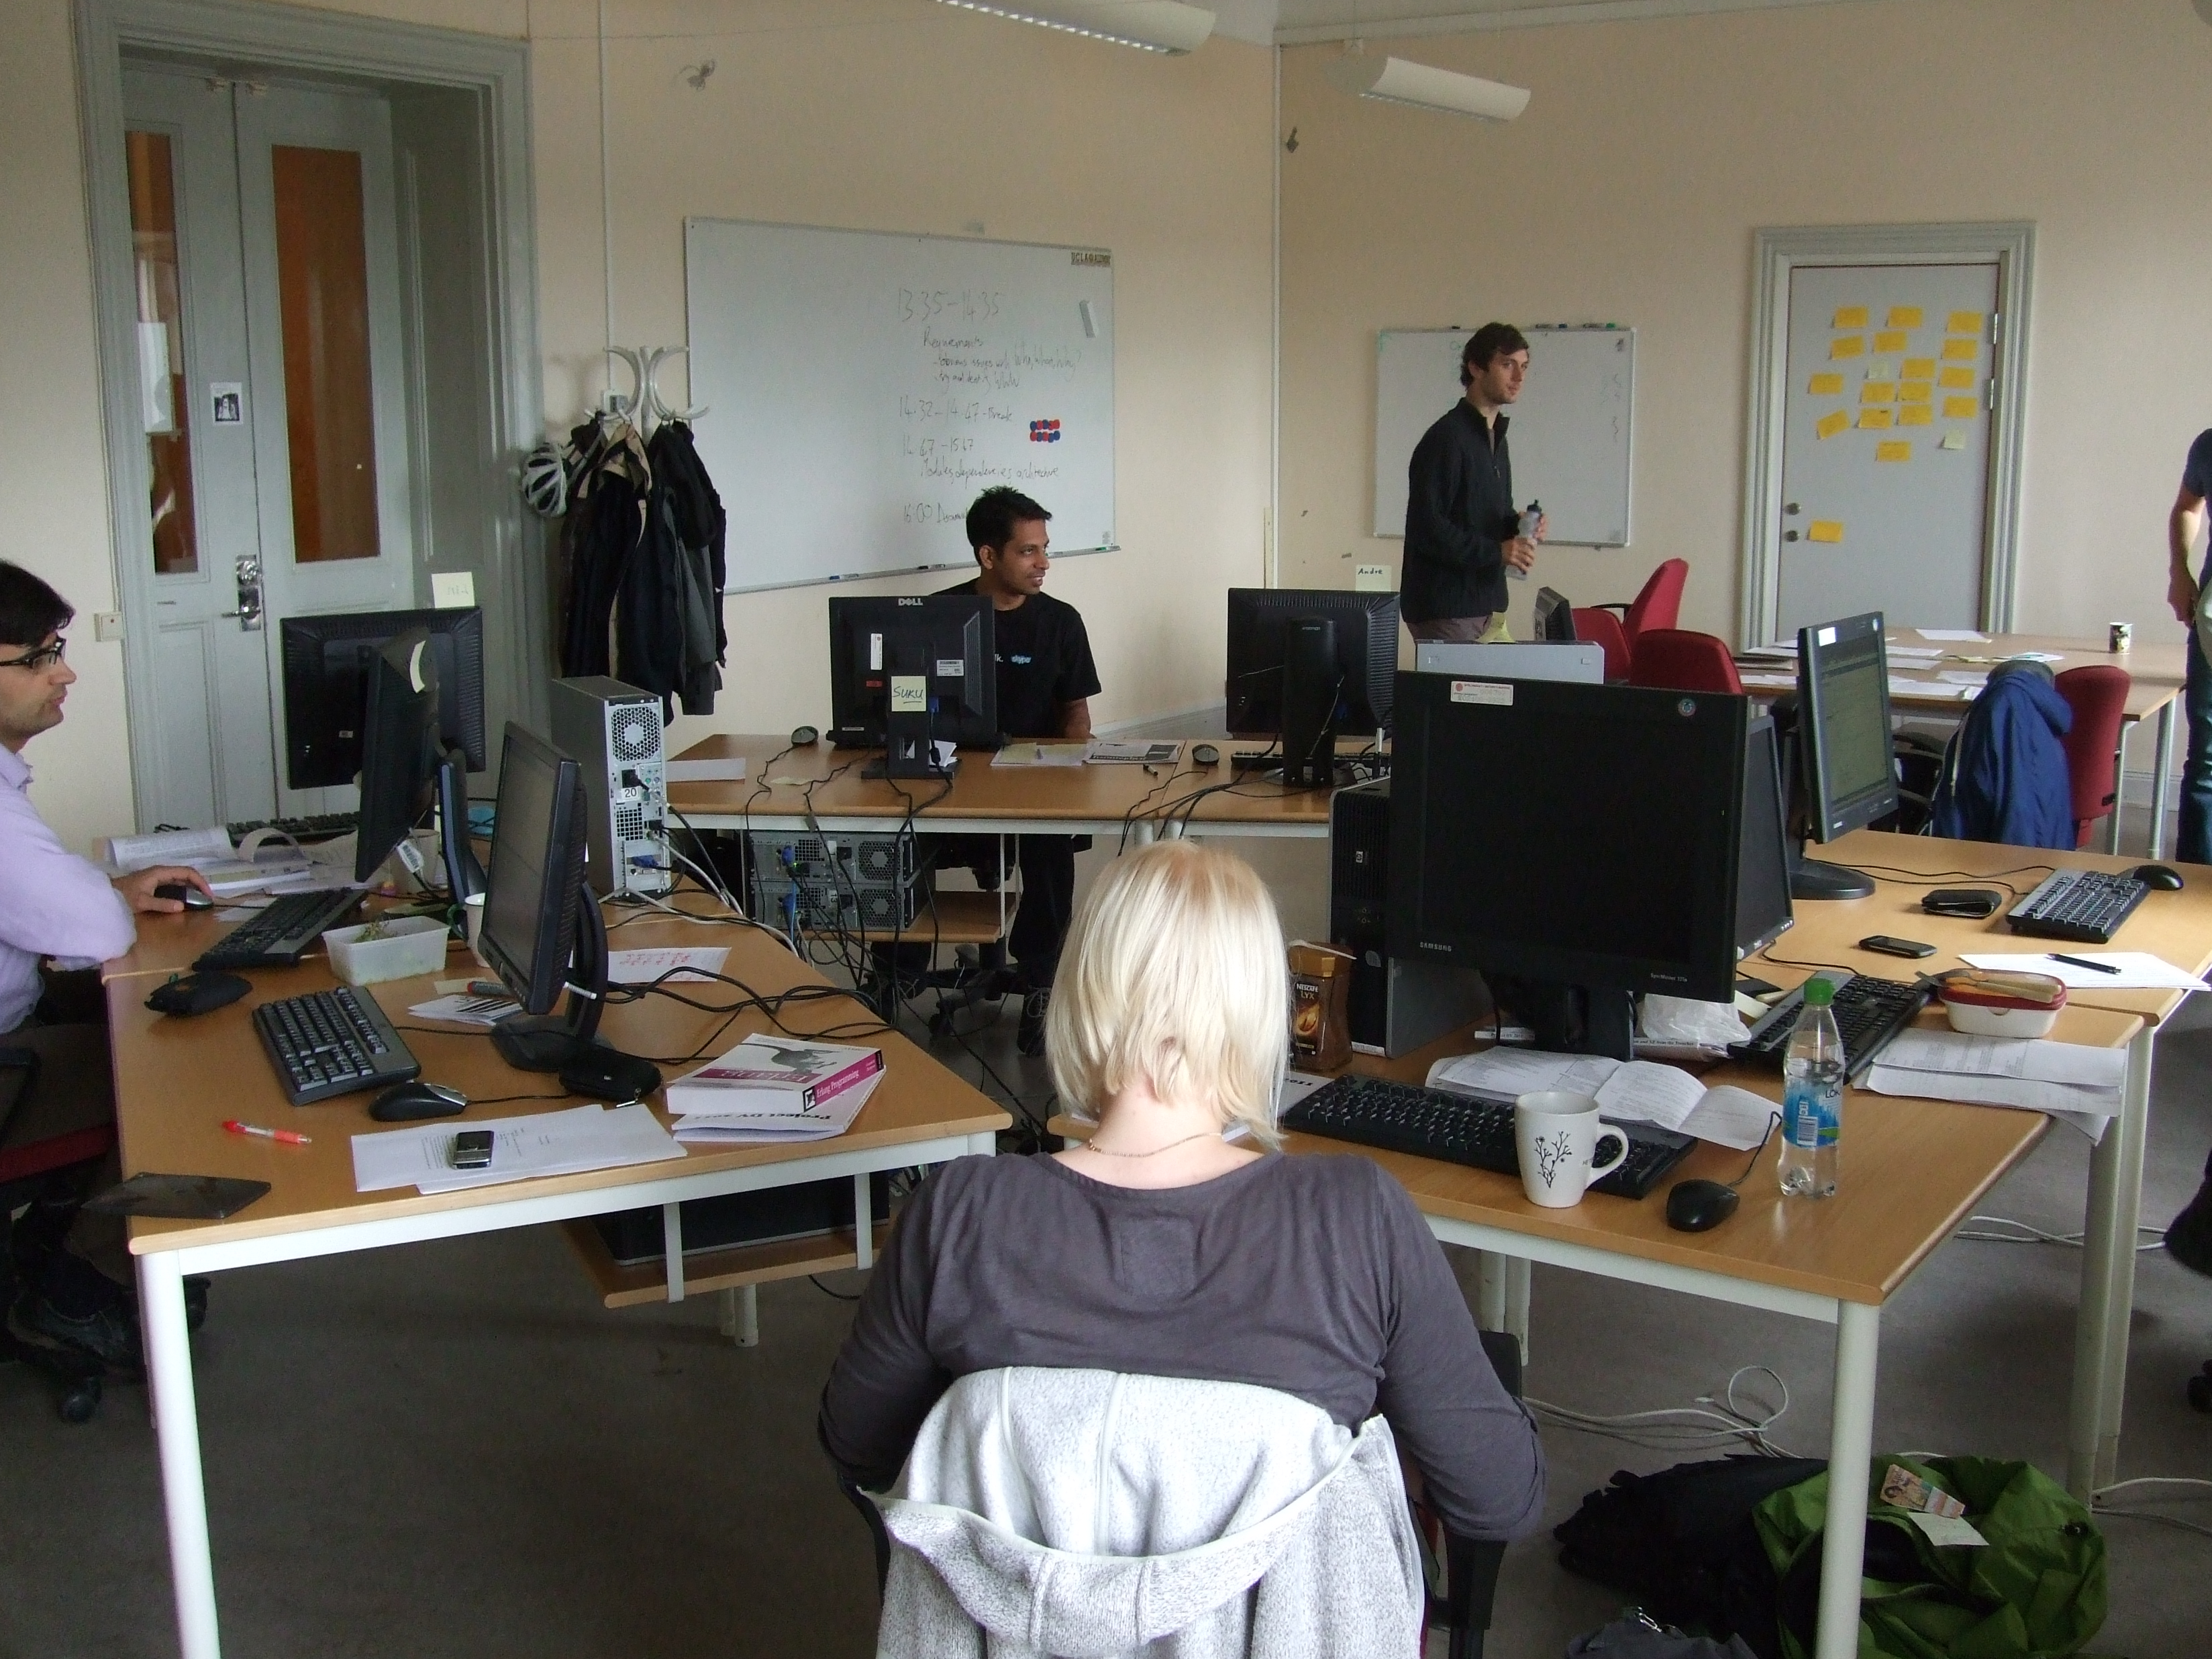
\includegraphics[width=12cm]{../presentation/images/diplomacy/DSCF6548.jpg}
 % DSCF6548.jpg: 3296x2472 pixel, 72dpi, 116.28x87.21 cm, bb=0 0 3296 2472
 \caption{Our Office}
 \label{fig:office}
\end{figure}


Even though we differed in nationalities as well as ages, we had no
troubles whatsoever to work together from the start.\\
\\
The team members were: \\

\newcommand{\flag}[1]{\includegraphics[height=10pt,width=15pt]{flags/#1}}

\begin{tabular}{lcrl}
Dilshod Aliev & Tajikistan & \flag{tajikistan.png} \\ \hline
Jan Daniel (JD) Bothma & South Africa & \flag{south_africa.png} \\ \hline
Stephan Brandauer & Austria & \flag{austria.jpg} \\ \hline
Andre Hilsendeger & Germany & \flag{germany.jpg} \\ \hline
Rahim Kadkhodamohammadi & Iran & \flag{iran.png} \\ \hline
Xinze Lin & China & \flag{china.png} \\ \hline
Tiina Loukusa & Sweden & \flag{sweden.png} \\ \hline
Erik Timan & Sweden & \flag{sweden.png} \\ \hline
Sukumar Yethadka & India & \flag{india.png}
\end{tabular}\\
\\
A list of the team members would not be complete without mentioning
Karl Marklund, the TA overlooking our project.
Karl has been a great help with all kinds of problems, from getting more
hardware to giving us tips and feedback. Thank you!

\section{Equipment}
We had nine development PCs (HP made) supplied by the university, as
well as three more PCs as servers (Git, Redmine, Gerrit, Buildbot),
a meeting/presentation workstation, a fault tolerance testing PC,
and one PC as load generator for load testing.

Our office room was equipped with several white boards that proved to be
very valuable, especially in times where much design and architecture was done.
\section{Tools}
\subsection{Issue Tracking}
All projects need a system for tracking issues and planning. We opted to use one
of the more popular open-source solutions called Redmine\cite{redmine}, a
web-based issue tracker and project management system. Redmine was useful to us
for several reasons:
\begin{itemize}
\item Built-in wiki \\
  We used the wiki as a basis for high level documentation of things such as our
  architecture and design, guidelines, scrum process details, test flow results,
  our data model and many other things.
\item Scrum plugin \\
  Redmine has a plugin system and we used the Backlogs plugin heavily. It is a
  plugin designed to help teams using scrum. It was very valuable since it
  quickly replaced the post-it based scrum board solution while providing the
  same visual overview. The scrum master had to spend no time on keeping our
  issue tracker and physical scrum board consistent any more.
\item Forum \\
  We used it for discussions during the initial sprints.
\item Version control integration \\
  We used the version control integration mostly for connecting tickets in
  Redmine to the associated commits in our Git repository.
\end{itemize}
\subsection{Version Control}
Perhaps even more vital to a software development project is a good version
control system. There are several out there, but the most common open-source
ones are Subversion and Git. They are fundamentally different and we chose Git
since it has very good tool support and handles branching and merging very well.

Another plus for Git is Github, an online repository hosting service. Most
open-source software written in Erlang (including Erlang/OTP itself) is hosted
on Github. This makes the process of making modifications to upstream code a lot
easier since it is trivial to fork (create your own hosted copy of another
repository) repositories on Github.
\subsection{Continuous Integration}
Continuous Integration (CI) is the process of building, testing and integrating
software in a continuous fashion. In practice, you use a special software that
checks out a copy of your source code tree from a version control repository and
runs various commands manipulating that source tree, returning some result to
the developers.

Initially we installed Jenkins to do this since it is widely used. We tried to
integrate it with our code review system, but the plugins for doing that were
very unstable and crashed often. We set out to find another system we could use
and found Buildbot. Buildbot is a bit different from most other CI servers since
it is more like a framework than a finished product. You configure Buildbot by
writing a Python program describing what it should do.

When we got Buildbot running and working integration with the code review
system, the team almost started treating it as our tenth team member. It proved
to be valuable to have this since it allowed us to avoid integration problems
early on. Our combination of Buildbot and the code review system made it
impossible to merge anything to our master branch without passing all tests.
\subsection{Code Reviews}
It is well known that it can be very useful to review code when developing
software for a number of reasons. One is that it often catches bugs that can be
hard to find with regular testing, another is that it allows other developers to
get acquainted with your own code. While many development projects uses code
review in some fashion or another, we wanted to try a more formal approach to
see if it could help us improve our code quality.

We quickly settled on using the code review system Gerrit. It was by far the
easiest code review system to setup for Git. The idea was to combine continuous
integration with the code review system to ensure that developers pay attention
to the results from Buildbot and that the master branch always is buildable and
releasable. It works like this:

When a developer pushes a change to the repository, she can not push to the
master branch directly but only to a new branch in Gerrit. Gerrit then publishes
this change in a pretty web interface for everyone to see {\bf and} tells
Buildbot to run the tests with that change. Now the other developers can review
that change by either looking at the changed files in the web interface or by
pulling them to their local repositories and try them out. If a developer finds
a problem, she can insert comments directly in the web interface for the author
to see and give a negative review in order to prevent merging of the change.

When the author has reacted to those comments, updated her change and the
reviewer is finally happy, the reviewer can give the change a positive rating
and submit the change, merging it to the master branch.

We configured our system so that if Buildbot {\bf and} at least one reviewer
agree that the change can be merged, Gerrit will do so. This process proved to
be incredibly safe, many bugs were found very early and our build broke (could
not compile the master branch) only once during the whole project. Some team
members actually started to use this system to get early feedback on unfinished
code and this worked out pretty well. Even though Gerrit+Buildbot is not easy to
set up, we think that future teams could profit a lot by using something
similar. We really do think that this workflow has improved our product and that
the invested time payed off.

We also use this system for more than code. In fact, while this report is
written, it is being code reviewed as well in the same manner.
\subsection{Building}
Build tools are important, especially since bad tools tend to cause frustration
among developers. We started using the Erlang build tool Rebar from day one in
our project since it is the de-facto build tool in the Erlang community. Rebar
can do quite a lot of things besides just compiling code. It also helps us run
tests and create releases.

We spent many hours integrating code from external parties into our system, such
as the server parts of our frontends. The majority of the external projects was
buildable with Rebar, but not the major ones such as ejabberd and exmpp. They
use plain Makefiles and are not releasable since they are not proper OTP
applications. To our great pleasure we learned at the Erlang User Conference
that there are forked versions of these projects that are OTP compliant and can
be built with Rebar. We switched to these forked ones late in our project, and
it simplified and sped up our build system a lot.

One thing we did not fully understand in the beginning was the relationship
between applications and releases. We thought that having a separate release for
our backend and each of our frontends was a good idea. While this is a fully
valid way to do things, it made life more complex when we tried to deploy and
configure a whole cluster. In retrospective, we should have kept all our
applications in one release and then dynamically start the ones we want to be
running on a specific node. That would have saved us some time and gray hair.
\subsection{Unit and Integration Testing}
There are several test frameworks for Erlang, but we used the standard EUnit
framework for testing for pretty much everything. We did so without really
considering CommonTest, so we do not know whether that choice was optimal or
not. EUnit worked okay for us but we had some problems with it.

One problem is that EUnit assumes an automatic timeout of 5 seconds for all
tests. If a test takes a long time to run (not uncommon in our system - we're
talking to a database), this timeout can become really annoying since some tests
takes longer under high load. Often tests would fail on Buildbot that did not
fail on our local machines. This was mostly because of the Buildbot machine
running several builds in parallel, creating a high load on that system. To make
matters worse, EUnit does not seem to have one central switch to change that
default value but only lets you change the value for single tests.

Another problem with EUnit is that tests often gets highly nested with lots of
anonymous functions being passed around. This makes it confusing to read test
code and sometimes hard to find the real problem behind a failing test.

We also had integration tests for our frontends. Each frontend had a basic
integration test checking that a user could log in and maybe do a few
operations. We used Selenium for testing the web frontend, and it turned out to
work okay-ish even though it was hard to write good tests for our
Javascript-heavy web frontend.
\subsection{Load Testing}
For load testing we decided to use Basho Bench, which made it possible to run
load tests that were repeatable and produce graphs out of the given results.
Basho Bench would run our tests, which contains a number of user commands, for
example logging in, sending messages and playing games. To really push our
system, we could configure it to use a number of workers, which would run the
test in parallel, over and over again until a given amount of time has passed.
With the architecture our system has, it is possible to tune many parameters,
such as the number of applications, the distribution of them and the number of
workers each application has.

To test something that would make sense, to us and the customer, we needed to
find some kind of average user behaviour, to get more realistic results on how
many users our system could deal with. We also needed to stress test parts of
the system, to find what configuration is best for each application, such as the
number of workers and the distribution of the database (which many applications
use). We had the system distributed across multiple machines, to be able to
test all aspects of the distribution and we tried to run them during nights so
we would get a fair result and be able to see if the system degrades over time
or not.

With Basho Bench, we were able to change the configuration of our system, run
the load tests and get some results, which we then could compare to other
configurations and analyze. During load testing we were able to find both bugs
and performance bottlenecks.

\chapter{Project Methodology and Organisation}

\section{The Customer}
Our customer was Jan Henry Nyström from Erlang Solutions\cite{erlsol}. Henry's
job according to Scrum was to prioritise the tasks at hand and be at the
planning meeting. What Henry did instead was to act more like a teacher which
led to confusion on our side at the beginning of the project. Once we got
accustomed to that, we were able to work very efficiently for and with him.
Henry's experience in developing Erlang systems was extremely useful and we hope
that he learned a little bit through this project as well since some of our
tools were not known to him (in practice) before.
\section{Erlang User Conference}
We were invited to present our project in poster form at the Erlang User
Conference in Stockholm\cite{euc2011}. The attendance was free of charge for us
thanks to Erlang Solutions.

In Stockholm many people asked about the project, most questions were on a high
level, though. We did not get direct feedback that changed the project after the
EUC but the talks there were quite relevant to our project and therefore a big
help.

It was as well a very fortunate place for us to be as some companies that were
there are actively trying to hire young developers with Erlang experience.
\section{Scrum}
For managing our project we used Scrum as in~\cite{kniberg}.
We tried hard to start up a well functioning software process and believe that
we succeeded. Our flavour of Scrum looked as follows: \\ \\
\begin{tabular}{cc}
  when & what \\ \hline
  daily & standup meeting\\
  weekly & fika \\
  beginning of sprint & planning \\
  end of sprint & demo \\
  end of sprint & retrospective \\
\end{tabular}

\subsection{Standup Meeting}
The standup meeting was strictly limited in time: to 15 minutes (although we
rarely reached 15 minutes). The standup meeting was held at 9:00 sharp every day
except for some planning days. In the standup meeting, everyone was giving a
short overview of his/her last day and of the plan for this day: ``Yesterday, I
did \ldots, I had problems with \ldots; today, I am going to \ldots''.
The positive effects of this are quite subtle and it might be easy to think that
such a meeting is not really necessary, especially when everyone is in the same
room:

\begin{itemize}
\item it encourages people to talk about their problems!
  Problems are not something one should hide. Many easy solutions for seemingly
  big problems came out of this procedure.
\item people maintain an overview of the project state even in the parts of the
  project they have not touched in ages.
\item since everything is announced before-hand,
  (``today, I am going to \ldots''), bad decisions can be caught, the rule to
  always work on the most important item is enforced and so on.
\item the standup meeting is an ideal opportunity for the scrum master to team
  up people who don't really know what they should work on.
\end{itemize}
\subsection{Fika}
The Swedish tradition of having Fika was something that has been practiced by
several teams on this course before us and we unanimously voted to have weekly
Fika, too. Every Monday, one member of the team would bring cake or pastry and
we would eat together and have coffee or tea. This was a delicious way to get to
know the team better.

In order to make people punctual (or: in order to have more Fika!), we decided
that each time someone is late for the standup meeting, that person has to
bring one extra Fika (or ``punishment Fika'', as we called it).
\subsection{Planning}
Planning was our least favourite task but nonetheless a very important one.
Our typical planning day looked as follows:
\begin{itemize}
\item 9.00--9.45: {\bf estimation of available person-days,
  prioritising of backlog stories}\\
  Who will be missing? What else is coming up (presentations, EUC, etc.)?
  What do we want to accomplish in this sprint?
  What is most important to the customer? The customer was missing that task
  often, so we had to guess what Henry would think.
\item 10.00--10.45: {\bf breaking down stories into tasks}\\
  Splitting the big stories into smaller tasks that ideally do not depend on
  each other --- but that was often easier said than done.
  Also: setting ``definitions of done'' (DoDs).
\item 11.00--14.30: {\bf estimating stories}\\
  (with breaks!)
  Guessing how long each story would take with the additional information from
  task breakdown and DoDs.
\item 14.30--15.00: {\bf committing to sprint}\\
  Taking the prioritised, estimated stories and committing to as many as the
  available person days allowed.
\item 15.00--16.00: Fika
\end{itemize}

\subsection{Demo}
The demo was held at the end of each sprint. Since in Scrum to try to produce
something that is potentially shippable in each sprint, the demo is there to
ensure that. We invited teaching staff and customer to the demos and showed them
what we did in the last weeks. The demo was always a nice ending of a sprint for
us, because it is in a quite relaxed atmosphere and we were more proud of our
product than worried.

\subsection{Retrospectives}
The retrospective was the absolutely last thing of a sprint --- in a team
meeting we talked about what we liked about the last sprint, what we disliked,
and what we would like to do differently in the next sprint.

It was very important to focus on getting negative feedback at first, people
were generally reluctant to give it because they did not want to seem rude or
be criticised themselves. This is, why we had the rule in the first one or two
retrospectives, that everyone {\em has\/} to come up with at least one of each
category. This worked quite well and in the end, even negative feedback was
coming quite easily, although personal criticism was very rare if occurring at
all.

After we had collected the feedback (we collected it in form of post-its on a
whiteboard), we ``dot-voted'' --- everyone gets three or four votes and can
distribute them in the form of a dot over the negative items on the board.
Giving multiple dots to one item is allowed. We took the three items with the
most points and tried to fix them in the course of the next sprint.
\section{Quality Management}
\subsection*{Coding Conventions}
Our coding conventions were agreed on in sprint 1 and we enforced them through
code reviews. Obviously some things were overlooked but the code quality
doubtlessly profited a lot from that practice.
The coding conventions governed coding style (eg.\ max-80-char-lines, no
trailing white space) as well as Erlang specifics (eg.\ how to use {\tt catch}).
\subsection*{Reviews}
Reviews were done mostly by whoever had time. A good time for a developer to do
reviews was while Buildbot was testing her newest change. Sometimes, though,
reviews were requested or even traded: ``I'll review your change, if you'll
review mine''.

At first it was annoying to have to wait for some time before a change was
actually merged. After a while, though, we got used to the fact that nothing is
merged immediately and continued to work on the next task while our old one was
awaiting review.

Reviews were generally well meaning but that does not mean that we accepted bad
code quality. People tended to look away when a function was not documented here
and there but there still were plenty of negative reviews.
\subsection*{Testing}
We took testing very seriously and the considerable time we invested payed off.
A counting on December 7$^{th}$, 2011 showed that 47\% of code lines were
testing code. This big suite of tests made it incredibly easy to verify that a
change didn't break anything. If developers are secured by a solid test suite,
it is also easier to start working on code that is not so well known because one
always has a regression test suite that immediately highlights errors.

\section{Timeline}
\subsection*{Sprint 1 --- Sprint Goal: ``Getting Ready to Code''}
\subsubsection{Servers}
We set up a Git-server and a Redmine-server, Buildbot was not
a task in this sprint. We started off with JD as scrum master and Stephan as
spokesperson. Scrum was done on a whiteboard with post-its.
As we all were new to the process, it took us a little while to figure out how
to act.
\subsubsection{Surveys}
We tried out some tools/libraries and evaluated how they would fit
our project. The end result of that process was (see Appendix B for details): \\
\\
\begin{tabular}{r|l}
Ubuntu 11.04 & operating system                                   \\
Git          & version control                                    \\
Gerrit       & code reviews                                       \\
Riak         & database                                           \\
Nitrogen     & web framework                                      \\
Yaws         & web server                                         \\
ejabberd     & XMPP server                                        \\
gen\_smtp    & email server library                               \\
Chromium 14  & web browser with WebSocket\cite{websocket} support \\
Buildbot     & continuous integration server
\end{tabular}
\subsubsection{Git-School}
Since almost everyone was new to Git, Erik talked to some slides about Git and
we all did a couple assignments with Git afterwards.
The other team was invited as well.
\subsubsection{Requirements}
We worked on the requirements a lot: we clarified them, prioritised them and had
our customer sign off the outcome of this process. It was crucial, that the
customer was happy with the result since we knew that this result would shape
the rest of our project.
\subsubsection{Preliminary Architecture}
We opted for a reviewed architecture process and would highly recommend it to
future teams as well:

A group of people was working on an architecture proposal for a couple of days.
Then one person of that group walked a review~group through the result. The
review~group then took the requirements and tried to run them through the
architecture. This proved to be very effective but of course work-intensive.

Given the importance of the architecture, the amount of work was acceptable.
\subsection*{Sprint 2 --- Sprint Goal: ``CRU Users''}
\subsubsection{Continuous Integration}
We set up Buildbot. Making our build process compatible with Buildbot was a lot
of work and maintaining the build process was a task in all future sprints.

Even though Continuous Integration was a lot of work to get up and running, the
productivity bonus it gave us more than made up for it in the long run.

\subsubsection{Testing Competency}
Some team members had not much or no real experience in writing tests, no one
had experience in writing tests in Erlang. Therefore we chose to hold a
{\em testing school\/} much like sprint 1's Git school.

\subsubsection{Load Test Riak}
Since our first design drafts showed that Riak would be very central to our
performance, we decided that a quick load test of Riak was in order just to
ensure that it `works'. The results where not extremely surprising and therefore
we continued to rely on Riak.

\subsubsection{Interfaces}
We laid the foundations for our interfaces: HTTP (WebSocket), XMPP, SMTP.
The DoD was to have them answer a `ping' with a `pong' or anything comparable.

\subsubsection{Registering, Login, \ldots}
We gave users the possibility to register on our system, to login and to update
their user information. First connections from the interfaces down to the
database were made!

\subsubsection{Problems!}
After sprint 1 which went very well, we were a bit too careless in sprint 2's
planning, especially the estimation - we underestimated the integration of
all user interfaces into the system A LOT.
For this reason, we committed to too many stories and were not able to complete
them by the end of sprint 2. We vowed to not make this mistake again.

\subsection*{Sprint 3 --- Sprint Goal: ``Play a Basic Game''}
From this sprint on, JD resigned as our scrum master --- but he had warned us
from the beginning of the project. Andre replaced him with the beginning of
sprint~3.

\subsubsection{Erlang User Conference '11}

Attending the EUC'11 was on our agenda. For that we had to make a
poster, which had to pass several stages of reviews. This proved to be very
time~consuming.
\subsubsection{Refactor UIs}
Since the input channels (HTTP, XMPP, SMTP) had been developed in parallel in
the last sprint, they were full of code duplication. We changed that and as well
extended them greatly.
\subsubsection{Game Application}
Since we wanted to be able to play games, we worked hard on the Game
Application. This ranged from setting up games as user (stored in the DB),
changing their phases according to a timer to implementing the game rules.

\subsection*{Sprint 4 --- Sprint Goal: ``Find the Limits of Real Games''}
\subsubsection{Load Testing}
We applied high load to our system and measured where the limits are (and how
they look like). The load tests showed us severe but easily fixable bugs that we
had in our system; we would not have found them otherwise. The scalability was
quite satisfactory for a first try, the raw performance however was degrading
over time until after $\approx$1h the backends crashed. We fixed this easily by
a reconfiguration of Riak but did not figure out exactly where the problem came
from.
\subsubsection{Messaging}
The messaging-part explains the word ``Real'' in the sprint goal since one
cannot play a good diplomacy game without communicating.

The messaging system needed to support offline messages (when a user receives a
message while she is offline, the message should be delivered upon login).
\subsubsection{Fault tolerance testing}
We needed a (semi-) automatic way of testing fault tolerance, since distributed
functionality like that is not possible to test with EUnit and can be quite
tedious. So we installed some VM containers on one of our servers, that could be
used to run multiple instances of the system on one machine. The goal for this
story was to provide the testing framework, not the fault tolerance itself, as
this would have been too much. Our System- and Cluster Managers are a byproduct
of this. They simplify the setup and start of a cluster by a great deal.

\subsection*{Sprint 5 --- Play game \& Operator is watching}
\subsubsection{Review 2}
Each team had to present their results, including a short demo. Both teams, the
teachers and the customers were present at those presentations. Additionally
some reviewers from the university and other master students were invited.

This was, like the EUC poster, very time consuming. Since we did not just
prepare the demo and the presentation, but we also had a test run, where Henry
Nyström and the teachers were present to give us feedback on the presentation.

We kept it quite non-technical, so that the end presentation could be mostly the
same.

\subsubsection{Tune performance}
After load testing in Sprint 4 we discovered that the performance of our system
was degrading over time. The DoD for this story was quite vaguely, as you are
never done tuning - and it's just fun! So we decided to solve the degradation
and if there is time left to tune performance, but not to spend more than 20 man
days on that story.

Our Riak storage backend was eleveldb, because it is the only one supporting
secondary indices. The assumption was that eleveldb, was responsible for the
degradation. The reason for that assumption was that Riak in general does not
show such a degradation pattern, and the default and well-tested storage backend
is bitcask. After replacing all uses of Riak's secondary indices with Riak
Search we could switch our backend back to bitcask.  This solved the degradation
problem.

Further performance tuning involved adapting the Riak write parameters.
Reducing these for the non-crucial writes, like message logging, was a simple
optimisation.

The last change regarding the performance was regarding another not so
well-tested Riak feature. On the \#riak IRC room on irc.freenode.net we got
the advice to try it without Riak Search. So we tried to remove it from as
many places as possible, and use Riak key filtering instead.  Load tests showed
this was indeed an improvement in performance.

Worth mentioning about the continuous load tests is that we discovered a drastic
performance drop due to some code changes. After a little while we could even
tell which commit was responsible and why. As it turns out it once again
increased the use of Riak search.

\subsubsection{Handle loss of servers}
We implemented the fault tolerance in the fifth sprint after providing the
testing framework for it in the previous one. This was achieved by our
necromancer module. Its responsibility was to watch nodes and react once a node
goes down. The nodes watched each other in circular manner, so that each would
be watched by one other node. Processes with state would simply write important
data to the database, and another node could then resurrect it with that data.

\subsubsection{Operator/Moderator functionality}
Many of our requirements were finished by sprint 5 and the majority of the
backlog consisted of Operator/Moderator functionality. So we introduced these
user roles and implemented an access control list together with some
functionality requiring privileged access, like inspecting servers and games or
blacklisting users.

\subsubsection{Graphical map}
A rather small, but to us very important, feature of that sprint was the
graphical map for the web interface. The game was not really playable with just
the textual representation of the map. We decided to do this only for the web
interface, since the other interface are purely text based anyway, and this was
a good task for HTML5 canvas\cite{html5_canvas}.
\subsection*{Sprint 6}
The last sprint was very short and was just about finishing up - we did not even
have a real planning meeting. We wrote all required reports (including this
one), published our project on Github, and fixed some bugs. We did not
introduce any new features whatsoever.

\chapter{Conclusion}
\section*{To Future Students}
\begin{itemize}
\item Investing in code quality pays off. Do never, ever, say things like:
  ``commit this now, we can make it pretty later''. Because you won't!  Do it,
  it's now or never.
\item Think `product': everything you do is in order to make the product better.
  You write high quality code because it makes you more productive, not because
  it's cast in stone.
\item Make everyone understand what you are talking about and take your time to
  do that.
\item Create an environment where it's ok not to know something so that people
  ask instead of trying to cover their problems. Help each other out where you
  can.
\item Planning is boring, but still: take your time to do it! It is incredibly
  motivating to see that a sprint goal was met after three weeks of hard work.
\item Work transparent: let everyone know what you are doing and why. This way,
  you get a lot more valuable feedback and no one can tell you later that what
  you did was wrong --- because they knew what you did.
\item Apply Scrum completely and take the time to read the material on Scrum and
  learn how to apply it properly. Don't feel bad for saying ``no'' to
  TA/customer if you are running out of time and you didn't commit to something.
\item It is good to have the same Scrum Master during several sprints, as he/she
  will get more comfortable in the role, but it is a team effort and if everyone
  knows what to do, the ``job'' gets easier. This is particularly important
  during the planning day, as the Scrum Master is leading the planning.
\item If your customer cannot be present during the whole sprint planning day,
  try to do the prioritisation while he/she is attending, as this is probably
  the most valuable thing for the customer during planning. This will also
  prevent you from guessing what the customer might want, and prioritising takes
  time!
\item Document early, document often. While this is not the most interesting
  aspect of coding, it definitely pays. Invest in your project's future by
  adding documentation.
\item Automate as much as possible. It always saves time in the long run.
\item Testing is your best friend!
      It saved us several times and makes people less reluctant to refactor
      or change other people's code.
      You can never have enough tests!
      $\sim 50\%$ of our code base was test code and yet we had bugs.
\item Do code reviews, they catch mistakes early and improve code quality.
      It is also one of the best ways to know parts of the system you are
      currently not working on.
\item Talk! Everyone is in the same room, often it's easier to just walk two
      meters, than having a conversation in a forum or the like -
      just don't talk too loud and disturb others!
\item Do Fika! Because it's delicious!
\end{itemize}
\section*{To Teachers/TA}
\begin{itemize}
\item We enjoy your visits and feedback!
\item It is great that you give the teams so much freedom.
\item The organisation of the course went very well, you were always helpful.
\item A little less report writing / poster making / presentation holding would
  make the product better and the course more fun.
\item Talks from industry experts would be very much appreciated.
\item It was hard for some of us to program using Swedish keyboards. Having
the option of English keyboards would be really helpful.
\end{itemize}


\section*{To wrap it up...}
This was a very fun, exciting and challenging course. We have gained new
knowledge in many areas, and something that was new to us all was the
language Erlang and the project methodology Scrum, we also learned to
use new tools and the importance of testing.

In a team like this, with students from different backgrounds in many regards,
from cultural to academical, it is important to respect each other and be
humble.  We really benefited from learning to know each other better through
fika and changing who we were working with on different tasks. We didn't enforce
pair programming, but those who felt more comfortable doing that had the
possibility to do it. In our working agreements we recommended team members to
eat lunch in the lunchroom, so we could have a casual chat.

Although, it has not been a breeze all the time. The project introduced
challenges in many regards, as there would be in any project. But we had
basically the same experience with Erlang, and we were more or less on the same
level in regards to that. Tools like Git and Gerrit were something new to parts
of the team, so there was a learning curve to many things. But in the end, we
all have something new to put in our bag of knowledge and experience.

\appendix

\chapter{Team Statements}

\section{Dilshod Aliev}
For me, as for other members of our team, the project has started with a survey.
I did a survey on the Nitrogen web framework: experimented with it and tried to
get it running on Yaws web server. It seemed to be quite suitable for our
project and, therefore, we decided to use it. However, later on it has been
eliminated from the list of tools we have been using in our project, due to some
problems. In addition to the survey, I spent some time on reading about Scrum
and attended Erik's Git School, together with other team members.

In the beginning of Sprint 2 I was supposed to work on the data model together
with Sukumar. Since I was new to the non-traditional databases, I spent some
more time on reading about key-value storage, Dynamo and Riak to have an idea of
how our data model should be designed. I am thankful to Sukumar for his help
and patience. In addition, during the Sprint 2 I worked on the user registration
and login parts of our initial web frontend.

In Sprint 3 I was working together with other members on different parts of the
system because I didn't feel confident to perform the tasks in a good way alone,
and to write clean, good quality code. However in the end of the sprint I
implemented some functionalities in SMTP client part. Furthermore I attended the
Erlang User Conference in Stockholm likewise other teammates.

During the first week of Sprint 4 JD and me worked on setting up SMTP
interface tests. Later I continued with implementing some functionalities like
viewing current games and searching for games using IM and Mail clients.
Moreover, I worked on the session and machine state so that the system operator
is be able to inspect the servers.

In Sprint 5 I worked on creating a graphical map for our game on the web
frontend. Later it has been integrated into our system by Lin. Afterwards I
spent some time on bug fixing and did some minor extensions to the IM and Mail
clients.

In the end, I would like to express my thankfulness to all my teammates for
being friendly and helpful. In addition, I recommend this course to students
who would like to experience a real project development in a team, and, once
selected, to help each other throughout the project and to create a good
teamwork environment.

\section{Jan Daniel Bothma}
During the first sprint I took on the role of Scrum Master, while also trying to
work as a normal team member. This was my first experience of Scrum so I spent a
lot of time learning about it and planning ahead to support the team as well as
possible. The rest of the team supported me a lot in this role.
I worked on grouping requirements from our Product Owner with Tiina
and Dilshod, and experimented with a custom WebSocket implementation.

In Sprint 2 I took part in developing our second architecture and high level
design. I made it as easy as possible to develop and run our code with ejabberd
using our automated build and test tools, despite our inability to build and
release it using Rebar. At the end of this sprint I gave up the Scrum Master
role to focus more on development.

In Sprint 3 I worked with Andre to guarantee consistency for some core
operations and implemented the solution for game joining in particular. I did
some further work on building ejabberd and improved our XMPP integration test
client.

I worked with Dilshod to set up SMTP integration tests and add them to our
automated test runs at the beginning of Sprint 4. Then Erik and I designed and
built the Cluster and System Manager applications to start up and stop a
distributed cluster of Treacherous Talks servers. I also implemented an Erlang
WebSocket client for our fault tolerance tests based on Yaws WebSocket code.

In Sprint 5 I implemented an automated test to check that games continue running
despite node or hardware failures. I presented this, and helped Rahim
demonstrate the working system at the Review 2 presentation. I then extended the
automated test to ensure all issues we had found with game resurrection were
fixed by Stephan and Tiina's refactoring.

I was home ill and unable to work for the first week of Sprint 6 and am very
thankful to the team for all their work on this and the Product Report.

\section{Stephan Brandauer}
I was the spokesperson of the team from the beginning. As spokesperson,
I saw it as my job to shield the team from distractions as much as possible.

In the beginning, I was doing the survey on Zotonic which looked great but too
big for us. Then, I also was part of the architecture team for the initial
draft.

My main topic in sprint 2 was Riak. I set up a cluster and was working with the
first benchmark of Riak, together with mostly Sukumar.
I committed the initial version of our DB-wrapper module as well.

In sprint 3, I was working on one task only: the rule engine, our implementation
of the rules. During that sprint, I got a lot done but also lost a lot of
overview over the project since I was working on one task, alone.

Sprint 4 started with the generation of test data for the load tests. After
this, my main contribution was necromancer, our fail-safety module as well as
integration of {\tt necromancer} in the system (Tiina did the implementation
of game-restarting).

Sprint 5 had me mostly covered preparing for the presentation of Review~2.
The feedback was quite good, but in my opinion we were forced to spend far too
much time on tasks that do not contribute to the product (I estimate that the
presentation preparation took roughly 3 person weeks).

\section{Andre Hilsendeger}
In the first sprint I was looking into Erlang Web as part of the tools-/library
survey. It turned out to be too basic and we did not use it. Additionally I was
part of the team that created the initial architecture draft.

As expected the initial draft of the architecture was not enough and needed more
specifics. In the second sprint I was once again part of the architecture/design
team. We defined in more detail what the processes are and how they are
supervised. As part of our testing school I also took a look into Meck, and gave
the team a short introduction on how to use it. Since by design most of our
backend apps had a similar structure I created a template for those and created
the initial user management app.

From the third sprint on I have been the Scrum Master. We noticed quite some
code duplications and similarities between our frontends, so I refactored the
logic away from the SMTP and XMPP frontends into the controller. Due to our
database-drive design in combination with Riak as our storage backend we had to
figure out how to maintain consistency. We identified the problems and tried to
solve them, adapting the controller to have a session process for every user was
part of that.

During the fourth sprint I implemented the event pushing to online users in the
controller, so that other apps, like the message-app, could push messages to
online users. After that I started my biggest and longest task, load testing. A
big part of that was to automatically setup multiple machines and run load test
on them, while Sukumar and Tiina wrote the actual load tests.

The results from the load test were not very satisfactory, so my task in the
fifth, and last real, sprint was to improve the performance. For that Rahim and
I replaced secondary indices with Riak Search, so that we could switch back to
the Bitcask storage backend. But as it turned out Riak search had serious
performance problems with often updated data.  So I replaces Riak search by key
filtering for parts of the system that did not really need the search feature,
like messaging.

\section{Rahim Kadkhodamohammadi}
In the beginning, I was doing some review on Erlang tools for SMTP and XMPP. In
this sprint Lin and me listed Erlang tools for SMTP and XMPP. I did some
experiments with the Mnesia database as well.

In the second sprint, I continued to do some experiments with ejabberd, the only
Erlang based XMPP server. I designed and developed an ejabberd component that is
able to exchange messages with users. Since EXMPP is the only Erlang based XMPP
client and we needed integration tests, I developed the first draft of an
application with EXMPP to do integration tests through the IM client. I was also
part of the architecture team.

Sprint 3 was the sprint where we provided functionality that allow users to play
games. During this sprint I mainly worked on the command parser, the controller
and the game application. I could say that it was a great sprint - I worked on
most parts of the system.

In sprint 4, I created our first draft of the message application which provides
functionality to send messages between users. Then I added the ACL (access
control list) to our controller. I also extended our web frontend to show some
system statistics to Operators and provide functionality to add/remove
Moderators.

In sprint 5, I was part of the presentation team. I was responsible to prepare a
demo to show during the presentation. I spent some time to prepare the demo and
fix some bugs which I encountered when played with our system. I also extended
our game and message applications to support black-listed users.

\section{Xinze Lin}
In the first sprint, I was surveying and experimenting with Erlang-based SMTP
servers for our project's need. Thanks to Erik's Git school and tool support, I
learned to use Git to commit my code to our repository.

In Sprint 2, I wrote the first version of our SMTP frontend server, which
enables email clients to communicate with the backend to register or update
users. The parser of the SMTP server was later refactored by Andre to support
both the SMTP and XMPP frontends at the same time. Beside that, with the help of
JD and Sukumar, I also created our code review checklist. And thanks to Stephan,
I learned the benefits of writing testing code.

During Sprint 3, I worked with Rahim on extending the parser and the controller
to support more user features. In addition, I extended the parser to support
Diplomacy game orders, which interprets the player orders from plain text to a
format compatible with our rule engine. Sukumar's Unix school made my life much
easier since I've never truly used Linux before.

In Sprint 4, I extended the web interface and backend to support in-game
messaging. I also did the operator web interface for inspecting database
status. With some help from Sukumar, I polished the web-interface a bit.

In Sprint 5, I created the Operator interface for inspecting the details of a
game. Also, I worked with Dilshod to make the game map usable on our web
interface.
\section{Tiina Loukusa}
In the first sprint, we were supposed to find out what tools and existing
open source software to use, I had a look at the web servers Chicago Boss and
Mochiweb, the database CouchDB and a bit at Zotonic along with Stephan.

In sprint 2 and after the first architecture was done, we found that we
needed to look into it in more detail. I joined the architecture/design team
later on to work on finding out what types of Erlang behaviours would be
suitable where and what the supervision should look like. Other than
architecture, I also worked on connecting a user through the web interface to
the backend.

In sprint 3 I was mainly working on the backend, and more specifically things
related to the game, games are started when they are created and processing of
game changes, so that the games progress properly.

Sprint 4 and 5 involved adding some operator and moderator functionality, such
as getting an overview of the state of the running backends and communication
between operators/moderators and users. I was also working a little with Sukumar
and Andre on the load testing, mostly figuring out what to test, but then we
noticed that three people are too many for that and I continued working on other
tasks.
As fault tolerance was a part of sprint 4, I made sure that games were restarted
properly, with the help of the necromancer which Stephan had implemented, and
thanks to JD who was working with fault tolerance testing this could be tested
properly.
\section{Erik Timan}
I wanted this project to have good tool support so I was elected to be the
system administrator for the team. I was very busy with administrative tasks in
the beginning such as installing the needed software on our servers. The team
opted to use Redmine for issue tracking and planning, Gerrit for code review and
Buildbot for continuous integration. It took me a while to get everything up and
running and I needed to hack some of the tools to support our workflow better. I
also held schools on Git and Redmine which took me a while to prepare.

I started working on the actual codebase during sprint 2. I took charge of
creating scripts for building and testing our system. Since we needed to
integrate code from external projects into our product and many of them were
quite painful to build, this was not as easy as we initially thought. By the end
of the sprint, most things worked and we could create releases of our system.

Initially in sprint 3 I worked with the poster that we would present at the
Erlang User Conference. Tiina and I worked together on first draft of the
poster. We got lots of feedback on our poster drafts and I spent quite some time
improving it. Later in the sprint I worked on reducing the build time for our
product since the long build times was making development slower. I also worked
on integration tests, game orders and various build improvements during this
sprint.

For me, the fourth sprint was mostly about making our releases actually work,
system configuration and fault tolerance testing. I created a proper staging
environment using the configuration manager Puppet. This allowed us to have
several light-weight virtual machines (containers) for fault tolerance testing
in a very easy and automated way. I then worked with JD on fault
tolerance testing. We reached a point were we needed an easy way to configure a
cluster of machines running various parts of our system. We created the cluster
and system managers as the cure to those problems. By the end of the sprint we
could actually deploy our system in a distributed fashion very easily.

Since sprint 5 was mostly about wrapping up the product, most of my time was
spent on polish and fixes. I added proper logging to the system and rolled our
different releases into a single one. I spent time on getting our integration
tests to actually use the cluster/system managers to control the system since
this got rid of lots of false positives that we got on Buildbot. I spent several
days on bug fixing our build-test-release cycle since we were hitting all kinds
of weird bugs during testing. I also spent a few days on trying to fix problems
found by Dialyzer in our codebase as part of the general clean-up.
\section{Sukumar Yethadka}
Building large scale Internet systems and its challenges are very interesting to
me, which is why, this project along with its requirement of ``Erlang for
everything" was an ideal fit.

During the initial survey sprint, I looked at various open source applications
(Yaws, ejabberd, Chicago boss) and tested to check if it worked with the kind of
usage we had in mind. I created slides for the Unix school with help from
Andre. I also helped create the coding guidelines and code review checklist.

Sprint 2 mostly involved working with the database. I did some basic read up on
Riak, learning how to use it efficiently. Then, I created the data model for the
system, updating it as per team feedback. I tested the data model with basho
bench thus making sure that Riak was a good starting point as the database. I
also provided feedback and suggested improvements to the initial version of the
architecture.

During sprint 3, I worked on the web frontend. After holding the Unix school, I
refactored the web frontend making it more modular, consistent and easily
extendible. It could have been better if we had used a traditional MVC
framework, but we decided to keep it simple making it Javascript heavy.

I worked on Riak search and load testing during sprint 4. I setup Riak search
and setup the search schema for the buckets. I also got it to work with the web
frontend. During the later half of the sprint, I worked on defining and creating
load tests along with Tiina and also created good visuals for the load test
results, using a open source project - highcharts.

With most of the core features completed, I worked on adding the less important
features, fixing bugs, cleaning code and fixing the documentation during sprint
5.

Overall, this project was a unique and memorable experience for me and is
definitely a recommendation for future students.
\chapter{Survey}
After a brief survey in the early stages of the project, we chose a few projects
to look at in more detail, to be able to make a fair decision on what might be
suitable for the Diplomacy server. As a reminder, all the projects mentioned
below are based on Erlang.

\section{Web Frameworks}
\subsection{Zotonic}
Zotonic\cite{zotonic} is a CMS based on Erlang. It has a powerful control
interface, has quite a number of modules available such as authentication and
chat and it achieves modularity by following OTP principles. Zotonic has support
for WebSocket and when WebSocket is not supported by the browser, it will
use Comet instead. Zotonic has been inspired by Nitrogen and it can only be run
on a MochiWeb server.

\subsection{Erlang Web}
Erlang Web\cite{erlangweb} is quite simplistic, it has support for multiple web
servers and distribution. It does not have any extras like a chat nor does it
have support for WebSocket. Erlang Web can be run on INETS and Yaws web
servers.

\subsection{Nitrogen}
Nitrogen\cite{nitrogen} uses an event-driven model and offers hot code swapping,
stability and scalability. It includes a simple, yet powerful, template system
and is well documented which is important for us as developers. Nitrogen can run
on several web servers; MochiWeb, Yaws and INETS.

\subsection{Chicago Boss}
Chicago Boss\cite{chicagoboss} is a new web framework, which has not yet reached
a stable state. Even though it hasn't reached 1.0, it still offers some nice
features, as it supports multiple databases, hot code swapping and e-mail among
other things. It is well documented but it does not support WebSocket nor
distributed systems.

\subsection{Results and discussion}
When we tried to decide on what web framework to use, we wanted simplicity, as
we had already decided on not to focus on the look and feel and we didn't want
to spend a lot of time on learning a specific web framework.
The project required the use of WebSocket and if the framework didn't
provide that up front, we would need to implement it ourselves.

Chicago Boss was too immature to be an option, as we want something stable that
we won't need to patch up too much and Erlang Web was very basic and didn't
provide many features that we could use, compared to the other ones.

The only web framework that had support for WebSocket was Zotonic, but it was
quite complex to learn to use it, and it didn't provide the kind of simplicity
we were looking for. We came to the conclusion that it would be of more use to
us to use a web framework that was easy to use and implement WebSocket support,
rather than learning how to create new modules for Zotonic.

We initially decided to use Nitrogen, because we found that it was one of the
more mature and well used web frameworks out of those we looked at. It could
work with both of the web servers we were choosing among, it was easy to use and
it provided some nice and useful features. It didn't have WebSocket support but
we thought we would be able to implement that.

Unfortunately, we came to the conclusion that implementing WebSocket support
into Nitrogen is a project on its own, and we decided to not use a web
framework at all. We ended up using only Javascript, which was sufficient for
our use.

\section{Web Servers}
\subsection{MochiWeb}
Mochiweb\cite{mochiweb} claims to provide a lightweight and lightning fast
web server. Several sources say that it has been used by Facebook for their
chat\cite{fb_chat}\cite{fb_pres}, due to these properties. It is easy to set up
and get running. It was really hard to find any documentation, because there is
almost no documentation online, only the API that can be generated by edocs
which in retrospective should be quite intuitive. A big drawback for this
project was that it doesn't have support for WebSocket.

\subsection{Yaws}
Yaws\cite{yaws} is a high performance web server, which has a large and active
community and is thus regularly updated. It can be run in two different modes;
as a standalone application or as an embedded application. Their web page
provides a large number of example use cases and it is well documented, which
might be a reason to its large user base. Something that really appealed to us
was the fact that it actually had WebSocket support!

\subsection{Results and discussion}
Both contenders were good web servers and we chose to look into these two more
closely because Nitrogen, which was the web framework we chose to use,
supported both. We had to choose one, and the lack of documentation and support
for WebSocket in MochiWeb made us choose Yaws. WebSocket support was definitely
the deciding factor.

As the WebSocket protocol kept changing under the course of the project, we were
lucky enough to have JD in the team, who found WebSocket to be very interesting
and cool. He updated the WebSocket implementation in Yaws, and these changes for
WebSocket RFC 6455 are now included in the release of Yaws 1.92.

Yaws seems to have been a fairly good choice, but during the EUC we became aware
of another web server, Cowboy\cite{cowboy_pres}, which in retrospective,
probably would have been an even better decision as the developer for Cowboy is
very keen on having the latest WebSocket version at all times. Why we didn't
even consider it an option was because it was very new and it had just entered
early beta when we did the survey when we had more mature options to choose
from.

\section{SMTP Servers}
\subsection{Erlmail}
Erlmail is a complete email solution written in Erlang. It contains OTP
compliant SMTP, IMAP and POP clients and servers. According to our observation
of its source code, it didn't support encryption. In general, it seemed like a
complex piece of software.

\subsection{gen\_smtp}
Gen\_smtp is a SMTP server framework that can be extended in an OTP style
fashion. It includes only a SMTP client and server, which means it doesn't
include any email retrieval mechanisms like IMAP or POP. This makes it simple to
interact with. Besides, gen\_smtp supports SMTP SSL/TLS-encryption.

\subsection{erlang-smtp}
Erlang-smtp contains a client and a server for SMTP and POP3.
According to its author, it does not yet support encryption.

\subsection{Results and discussion}
Considering the fact that we only need a simple server to send and receive
emails, we didn't need much features except for SMTP protocol
support. Therefore, our architecture team voted for gen\_smtp for its
simplicity.

\section{XMPP}
We needed an XMPP server for providing that interface to our application, and a
client for testing it.

\subsection{ejabberd server}
ejabberd is a distributed Jabber/XMPP instant messaging server. It has a modular
architecture, a web administrator interface and simple configuration. It
supports extension via \emph{internal components} in the form of Erlang modules
using hooks which can be added allowing it to control the server in a
programmatic way\cite{ejabberd-plugin}. It also supports more advanced features
such as the Jabber Component Protocol \cite{xmpp-component} and a server to
server (S2S) protocol\cite{xmpp-s2s}.

\subsection{exmpp client}
\emph{exmpp} is a XMPP client with SSL support. It provides a lot of functionality to
deal with XML and supports several XML parsers. However, its documentation is
sparse.

\subsection{Results and discussion}
ejabberd was the only real option regarding XMPP server implemented in Erlang.

We had to choose how to interface our application with ejabberd, and decided
to use the internal ejabberd component form for its tight integration and
simplicity.

We used the exmpp client later in the project for integration
testing since it is easy to script test cases using the IM interface.

\section{Databases}
\subsection{Mnesia}
Mnesia is a distributed relational database designed for telecom systems and is
a part of the Erlang/OTP distribution. It is a well documented, fault tolerant
database that provides the ACID\cite{ACID} guarantees of Atomicity, Consistency,
Isolation and Durability and supports dynamic reconfiguration as well
as transactions. However, it has a storage limit of 4 gigabytes and has a
learning curve of its own custom query language.

\subsection{Riak}
Riak is a distributed key value database based on the CAP
theorem\cite{cap_theorem} and Amazon's dynamo paper\cite{dynamo}. It provides
features such as RESTful interface, protocol buffers interface, ability to tune
CAP values at the bucket level, map reduce queries, link walking, secondary
indicies and search. All the data is replicated across the nodes based on the
configuration without the usage of a master node. It is fault tolerant and built
with horizontal scaling in mind. Riak, by design, is eventually consistent.

\subsection{CouchDB}
CouchDB is a distributed document oriented database and is quite similar to Riak
in terms of its feature set. Its differentiating factors are that the document
is stored as a JSON object, it is ACID compliant, uses Multi-Version Concurrency
Control (MVCC) and has indexed views providing fast queries. Also unlike Riak,
each node of CouchDB stores the entire dataset and it has the concept of a
master node.

\subsection{Results and discussion}
The initial thought we had when starting off with the project was that in order
to make our system scalable and fault tolerant, we need to reduce the amount of
state in our backend as much as possible. This resulted in a database driven
architecture, making our choices more specific.

While Mnesia was a good option, it was not linearly scalable due to its
transactions. In order to keep the data consistent, Mnesia uses transactions
that lock up the data until all the copies in all the nodes are updated.

CouchDB was also a good option, but because it stored all the data in all the
nodes and had a single point of failure - the master, we couldn't use it.

Riak, with all its features and documentation, seemed like a perfect fit for
us. The main selling point for us was its advertised linear scaling and fault
tolerance. Basho releasing a stable 1.0 version during the survey helped as
well.

\renewcommand\bibname{References}
\bibliographystyle{unsrtnat}
\bibliography{course_rep}

\end{document}
